\documentclass[tikz,border=12pt]{standalone}
\usepackage[T1]{fontenc}
\usepackage{lmodern,amsmath,amssymb}
\usetikzlibrary{arrows.meta}
\definecolor{ink}{HTML}{183444}
\definecolor{blue}{HTML}{1B6780}
\definecolor{amber}{HTML}{AD601A}
\begin{document}
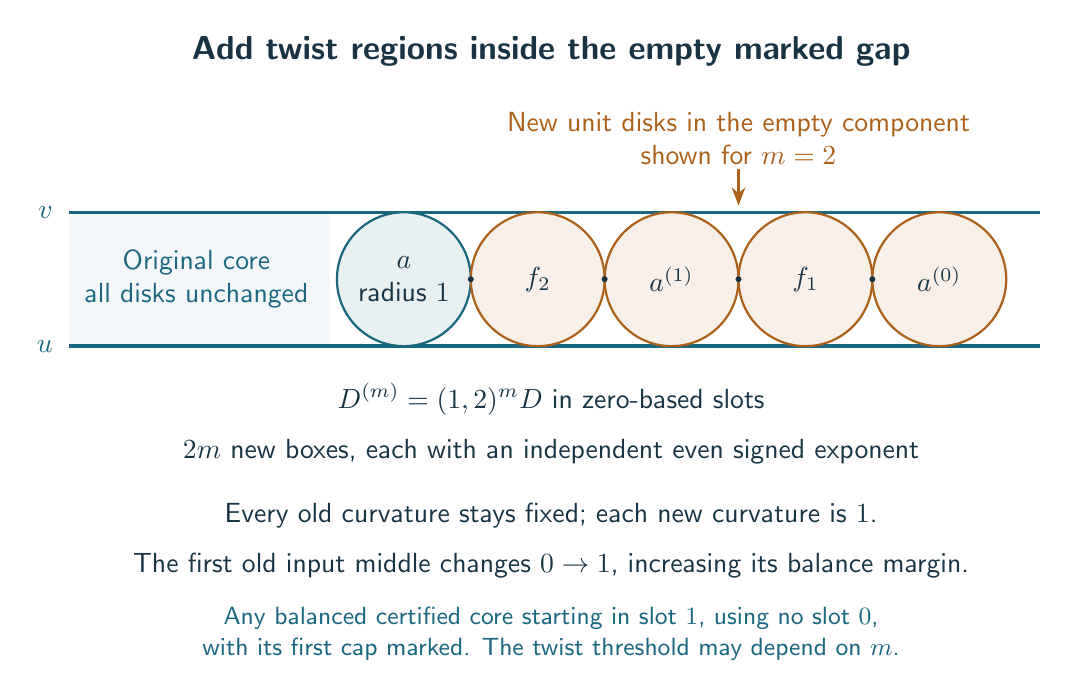
\begin{tikzpicture}[font=\sffamily,text=ink,>=Stealth,scale=.85]
 \node[font=\sffamily\large\bfseries] at (2.2,4.4)
 {Add twist regions inside the empty marked gap};
 \fill[blue!5] (-5,0) rectangle (-1.1,2);
 \node[align=center,text=blue] at (-3.1,1)
 {Original core\\all disks unchanged};
 \draw[blue,very thick] (-5,0)--(9.5,0);
 \draw[blue,very thick] (-5,2)--(9.5,2);
 \node[anchor=east,text=blue] at (-5.1,0) {$u$};
 \node[anchor=east,text=blue] at (-5.1,2) {$v$};
 \draw[blue,thick,fill=blue!10] (0,1) circle (1);
 \node[align=center] at (0,1) {$a$\\radius $1$};
 \foreach \x/\lab in {2/f_2,4/a^{(1)},6/f_1,8/a^{(0)}}{
  \draw[amber,thick,fill=amber!10] (\x,1) circle (1);
  \node at (\x,1) {$\lab$};
 }
 \foreach \x in {1,3,5,7}{\fill[ink] (\x,1) circle (.045);}
 \node[align=center,text=amber] at (5,3.1)
 {New unit disks in the empty component\\shown for $m=2$};
 \draw[->,amber,thick] (5,2.65)--(5,2.1);
 \node[align=center] at (2.2,-1.15)
 {$\displaystyle D^{(m)}=(1,2)^m D$ in zero-based slots\\[6pt]
 $2m$ new boxes, each with an independent even signed exponent};
 \node[align=center] at (2.2,-2.9)
 {Every old curvature stays fixed; each new curvature is $1$.\\[6pt]
 The first old input middle changes $0\to1$, increasing its balance margin.};
 \node[align=center,font=\sffamily\small,text=blue] at (2.2,-4.3)
 {Any balanced certified core starting in slot $1$, using no slot $0$,\\
 with its first cap marked. The twist threshold may depend on $m$.};
\end{tikzpicture}
\end{document}
